% !TEX root = ../main.tex

% 第一章一般名为绪论/引言,不可省略

\chapter{绪论}

\section{研究背景}
随着计算机图形学、计算机辅助设计和多媒体技术的发展,三维模型越来越多地应用于人们的生产和生活中,并成为人们生活中不可或缺的一部分。三维模型被广泛应用于计算机游戏、电影和其他虚拟现实的应用中,通过对三维模型的渲染,人们可以看到逼真的图像,让我们获得美妙的视觉效果。随着虚拟现实技术的兴起,三维模型将成为一个越来越重要的角色。三维模型也被广泛应用与工业制造,都会通过计算机辅助设计先在计算机中生成三维模型,然后进行测试、修改,最后才投入生产。新兴的3d打印技术更是让这个过程变得更加便捷,让我们可以将大多数三维模型变成现实。
在计算机中,三维模型主要表示方式有两类:连续的表示方法和离散的表示方法。连续的表示方法如代数曲面可以很精确并以很少的数据量来表示一个简单模型的表面,但是对于很多模型很难找到一个曲面的解析表达。因此,在计算机中我们常用离散的三角形或多边形网格来表示一个三维模型,其中我们最常的是三角形网格表示法。
现在三维模型的主要来源有两个:(1)依靠计算机辅助设计,人工制造;(2)依靠3维扫描仪扫描之后重建得到。得益于3维扫描仪,三维模型种类和数量大增。现在三维模型不仅复杂度日益增加,而且对三维模型的细节和精度的要求也日益提高,更丰富的细节和更高的精度在使得基于三维模型的计算机应用带给我们更多的真实感,使得工业制造更加精准的同时,也使得3维模型数据量大增,使得对三维模型的存储、传输、显示、修改这些基本操做带来了相当大的困难,而且使得很多计算机图形学的算法的计算量也大幅度增加。而对于一般的应用需求,在很多时候并不需要高精度的细致的三维模型,因此在一个较低的误差范围内,用一个顶点(或三角面片)数量尽可能少的三角网格来近似原网格成为了一个迫切的需求。

%% 绪论第一节一般是研究背景,
%% 交待下这个领域遇到了什么亟待改善的困境。
%% 从严谨的学术观念考虑,必须引用足量的数据描述现状,
%% 避免使用过多主观判断的语句和用词。

\section{相关工作}

网格简化算法的研究已经有一段时间了,在相关网格简化算法之中常用的三角网格简化操作有消点,顶点聚簇合并,消边等。顶点的消点操作是指在消除一个三角形网格上的一个顶点以及包含该顶点的边和面形成一个洞,然后利用该洞的边界点的组合构成的三角形补洞(如图1.1)。顶点聚簇合并是指通过同时合并两个或多个三角网格上的顶点的方式来减少顶点和三角面片(如图1.2)。消除边操作可以看做是顶点聚簇合并的一个特例,要求一次只能合并构成一条边的两个顶点。
\begin{figure}[htbp]
    \centering
    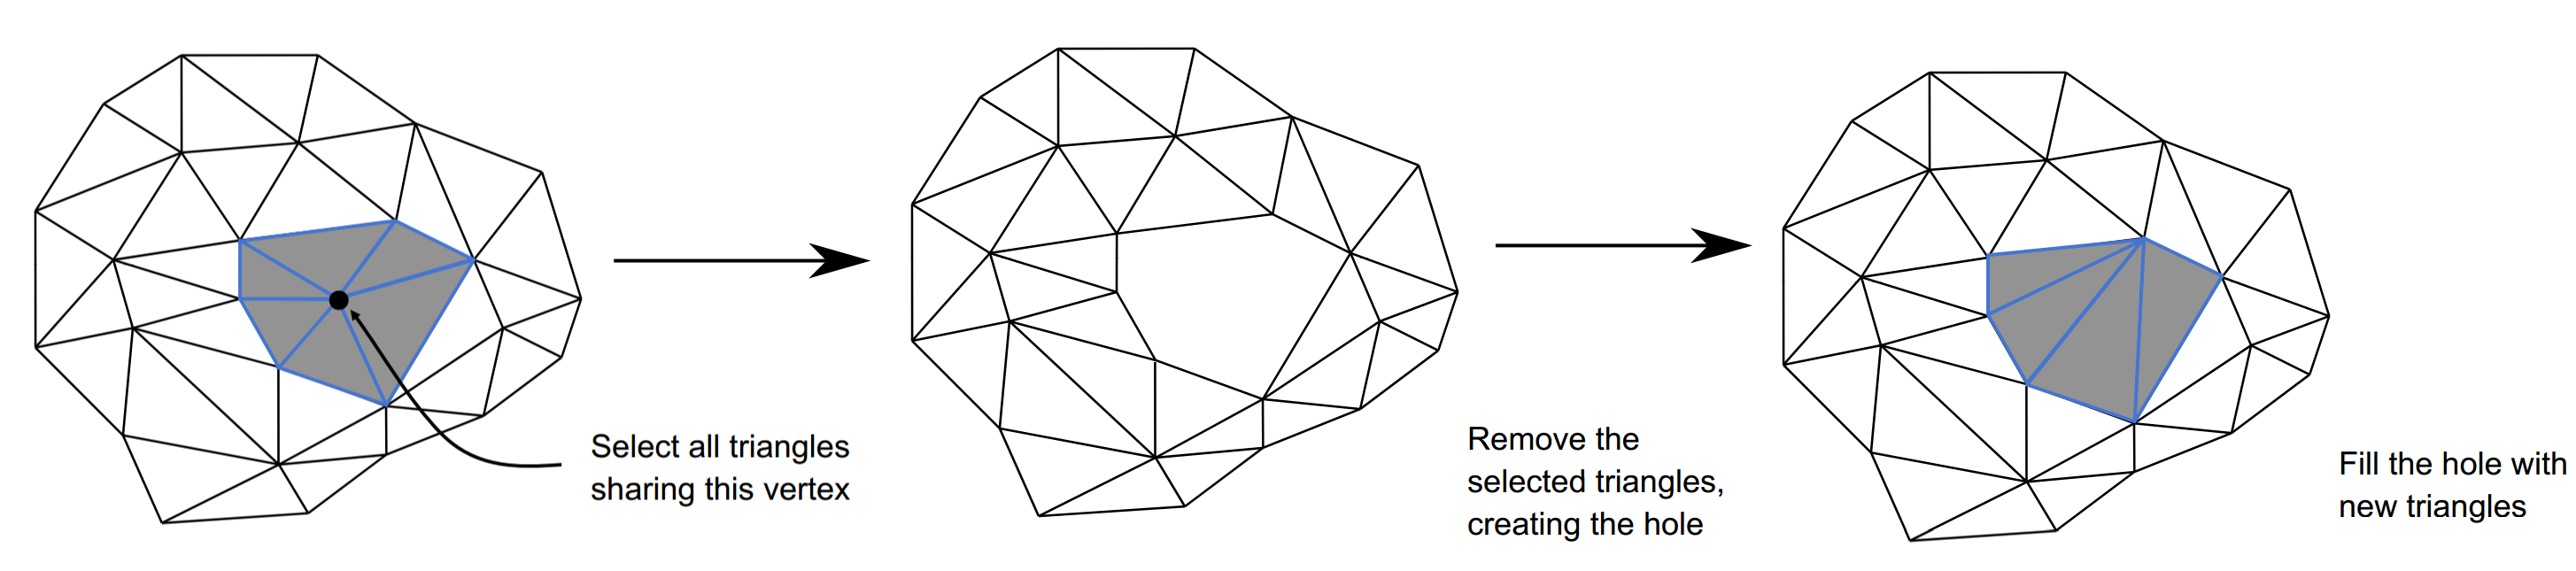
\includegraphics[width=.8\textwidth]{vertex_remove.png}
    \caption{通过顶点删除的操作简化网格,图来自\cite{mesh-simp}}
    \label{fig:顶点删除示意图}
\end{figure}
\begin{figure}[htbp]
    \centering
    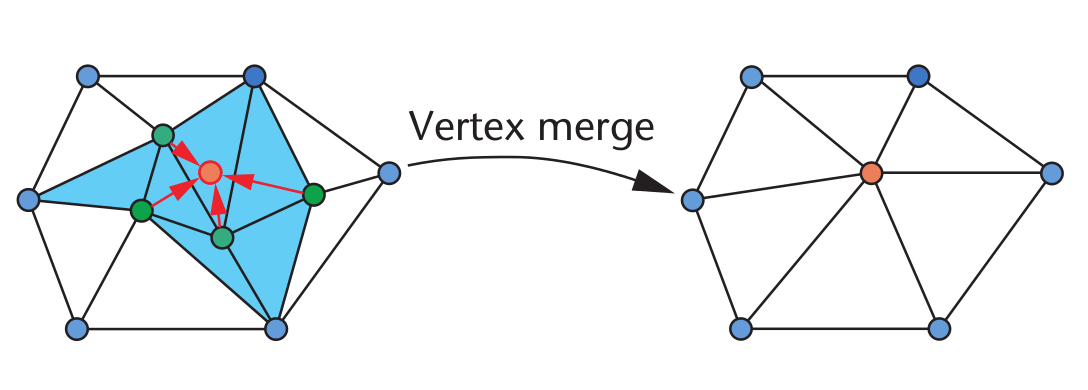
\includegraphics[width=.8\textwidth]{vertex_clustering.png}
    \caption{通过顶点聚簇合并的操作简化网格,图来自\cite{mesh-simp}}
    \label{fig:顶点聚簇合并示意图}
\end{figure}
%% 对于国内硕士学位论文来说,
%% 一般较少研究完全无前人探索的领域,
%% 所以有必要交待前人在此做出的努力和尝试。
%% 同样,请提供数据和引用保证严谨。

%% 为避免引起评阅老师判定有凑篇幅之嫌,
%% 请有针对的描述前人研究的不足之处,
%% 做到``有破有立''。
%% \def\theequation{S\arabic{equation}}
在网格简化算法中,我们通常用Hausdorff距离被用来作为衡量简化结果与原网格之间的误差(以下Hausdorff距离公式,引用自$https://en.wikipedia.org/wiki/Hausdorff\_distance$)。单个
点$x\in\mathbb{R}^3$到一个三角网格$F$的 Hausdorff 距离定义为:
\begin{equation}
d(x, F) = \underset{y\in F}{inf}||x-y||
\end{equation}
这里y是三角网格F表面上的任意一点,inf表示取最小值。定义三角网格$F_1 \to F_2$的最大Hausdorff距离为:
\begin{equation}
  \rho_{max}(F_1,F_2)=\underset{x\in F_1}{sup}(x,F_2)
\end{equation}
这里sup表示取最大值。定义三角网格$F_1 \to F_2$的平均Hausdorff距离为:
\begin{equation}
  \rho_{mean}(F_1,F_2)=\underset{x\in F_1}{avg}(x,F_2)
\end{equation}
这里avg表示取平均值。定义三角网格$F_1 \to F_2$的Hausdorff距离的均方根(RMS)为:
\begin{equation}
  \rho_{rms}(F_1,F_2)=\underset{x\in F_1}{rms}(x,F_2)
\end{equation}
定义两个三角网格之间的双向最大Hausdorff距离和双向平均Hausdorff距离以及双向Hausdorff 距离的均方根分别为:
\begin{equation}
  \begin{array}{l}
    d_{H\_max}(F_1,F_2)=sup(\rho_{max}(F_1,F_2), \rho_{max}(F_2,F_1))\\
    d_{H\_mean}(F_1,F_2)=sup(\rho_{mean}(F_1,F_2), \rho_{mean}(F_2,F_1))\\
    d_{H\_rms}(F_1,F_2)=sup(\rho_{rms}(F_1,F_2), \rho_{rms}(F_2,F_1))
  \end{array}
\end{equation}
相同的Hausdorff距离下,比较网格的简化程度(顶点或三角面片数量),或者相同的简化程度下比较简化之后的网格和原网格之间的Hausdorff距离是比较两个网格简化算法的重要依据。根据给定不同的网格简化条件,当前的简化算法可以分为两类:$Min−\#$类算法和$Min−\varepsilon$类算法。$Min−\#$类算法给定一个误差范围ε以及其计算方式,在保证简化的结果与原模型间的误差不允许超过ε的条件下做网格简化。$Min−\varepsilon$类算法则在给定一个最终的简化结果的顶点或三角面片数量的条件下,尽可能地最小化简化结果与原网格之间的误差。\par
在所有$Min−\varepsilon$类简化算法中,Michael Garland等人提出的QEM算法\cite{qem}凭借其高效简单效果好,成为较流行的网格简化算法之一。现在,我们可以下载到实现该算法的开源应用QSlim。在该算法中,每个三角网格模型被视为是由很多个有限的平面所构成。该算法的主要思想是在做顶点合并时,最优化(最小化)每个顶点到其所属平面集合的距离平方和,从而将降低每次简化带来的误差。与该算法相似的还有Peter Lindstrom等人提出的MemorylessSimplification,也是通过贪心的策略迭代地合并顶点。与前者不同的是该算法将上一次的结果作为参考,最优化(最小化)的是新网格与参考网格所构成的体积。该算法通过这种保体积的策略,得到了比QEM算法更优的简化效果。由于在确定一个定点对的合并点位置时,需要最优化体积,因此需要消耗的时间是QEM的10倍左右。\par
为了满足在高精度范围内简化网格的需求,产生了$Min−\#$类算法,其中最具代表性的算法之一是Jonathan Cohen等人提出的一种基于内外壳的网格简化算法\cite{?}。在用户给定最大误差$\varepsilon$的条件下,该算法首先生成与原始网格距离为$\varepsilon$的内外壳边界,然后在保证新生成的三角面片不与内外壳相交的条件下做顶点合并。而在同样给定最大误差$\varepsilon$的条件下,Borouchaki等人提出了一种能够直接约束Hausdorff距离不超过$\varepsilon$的网格简化算法——MMGS,而且在MMGS中通过翻面和定点光顺优化了定点的位置,使得结果更加光顺。在2015的SIG上Manish Mandad等人发表了一种将网格重建和基于内外壳简化算法相结合的网格近似算法,该算法也是本文主要参考的算法。该算法能在给定内外边界采样点的情况下,先通过世面体化重建出一个夹在内外壳之间的原网格近似,在此基础上通过消边来简化这个四面体结构,从而生成一个尽可能简化的网格去近似原网格,我们将在后续的章节中详细介绍。
\section{本文工作}
通常我们以以下几个方面来评价一个网格简化算法:
\begin{enumerate}
\item 相同误差下简化程度的高低和相同顶点数量下简化误差的大小;
\item 能否较好地保持原网格的法向信息;
\item 算法是否高效简单。
\end{enumerate}
现在的一些主流的方法,虽然能够较好地满足一般用户的需求。但是均无法做到能够鲁棒地处理各种输入数据的同时能够严格地控制简化误差。而最近 Manish Mandad等人提出的网格同坯近似算法,很好地做到了前三点。我们在实现其算法的基础上,对其可能存在的不足做了分析,并实现了我们的改进。Manish Mandad等人提出的网格同坯近似算法大致可以分为以下几个步:细化、简化误差边界、镶嵌0等值点、简化0等值面和消除所有可能消除的边。该算法以在误差空间Ω的内外边界(内外壳)上密集的采样点S来作为输入数据,在细化阶段,以这些采样点的包围球的3D Delaunay三角化作为初始化,在这个三角化的每个四面体上维护一个线性差值函数,其中包围球和外壳采样点的值定为1,内壳采样点的值定为-1。然后不断地往这个三角化中加入内外边界的采样点,直到这个差值的0等值面(所有差值为0的点构成的面)能够将所有的内外采样点区分开,这样就得到了一个原误差空间的近似Γ。简化误差边界,就是在保持0等值面仍能够区分内外采样点的条件下去尝试消除误差空间Γ边界上的边。在镶嵌0等点,则是将所有在边上的0等值点插入到这个三角化中。在镶嵌0等值点之后,就得到了显示的0等值面——原网格的一个近似,不过这0等值面还不够简单,我们需要尝试消除每一条由0等值点所构成的边,在保持0等值面任然能够将内外采样点区分开的条件下。之后为了进一步简化,可以在该条件下,继续消除所有可能消除的边。由于该算法始终确保0等值面能将内外采样点分开这个条件,因此能够严格地控制误差。并且在整个简化过程中依次遍历所有可能消除的边,在消边时则通过对附近空间采样去寻找可能的合并点的位置,因此,在简化结果上,与以往的算法比较具有明显优势。然而,在初始化重构网格时用的3D Delaunay三角化,虽然这样能够拥有较好地质量,但并没有考虑到原三角网格本身存在的各项异性,从而使得接下来需要经过消边来获得这个特性。为了获得一个更好的初始化,我们需要一个各项异性的 3d delaunay 三角化。我们根据原三角网格的曲率信息,对其做一个形变,在形变空间中做3D Delaunay三角化,对应到原空间中我们就得到了一个各项异性的三角化。这样的初始化,不仅大大简化了细化的结果——得到了一个更好的初始化状态,而且使得最终我们能够在给定的误差范围内得到一个顶点数量更少的结果。
%% 此部分必须详细描述,
%% 必要时可划设小节。
%% 国外学位论文的Introduction章基本仅阐述此内容。
%% 为研究开展的相关工作和实验,
%% 此间遇到何难处及对应的解法。
%% 对论文研究领域不甚了解的评阅老师,
%% 希望从摘要和此小节尽可能的了解最多信息。


\section{论文的内容和结构安排}
首先我们介绍了现阶段三角网格简化在计算机图形学和计算机辅助设计中的重要意义,以及现阶段三角网格模型简化的背景,并介绍了现在国内外的一些研究成果和算法以及它们各自的优势和不足。然后提出了我们认为的三角网格简化的几个目标,并介绍了我们改进的基于内外壳的网格简化算法及其具体实现。最后是我们对三角网格简化工作的总结和展望。\par
本文的章节安排如下,第一章介绍网格简化的背景和国内外对网格简化的研究现状,以及本文的主要工作;第二章对我们所参考的一些主流的网格简化算法做了一个详细地介绍和分析;第三章,详细描述了 Manish Mandad 等人提出的基于内外壳的网格近似算法;第四章,我们基于 Manish Mand 提出的算法的改进;第五章,我们的算法的结果展示;第六章是总结和展望。
